\documentclass[11pt]{article}
\usepackage{report}

\begin{document}
\section{Problem 1}
In appendix \ref{code:hatfun} we can see the code that implements the hatfun function. In order to see clearly how it works we have plotted the function for $n = 2,5,10$. Where n stands for the subscript in the hat function. 
\begin{figure}[H]
	\centering
	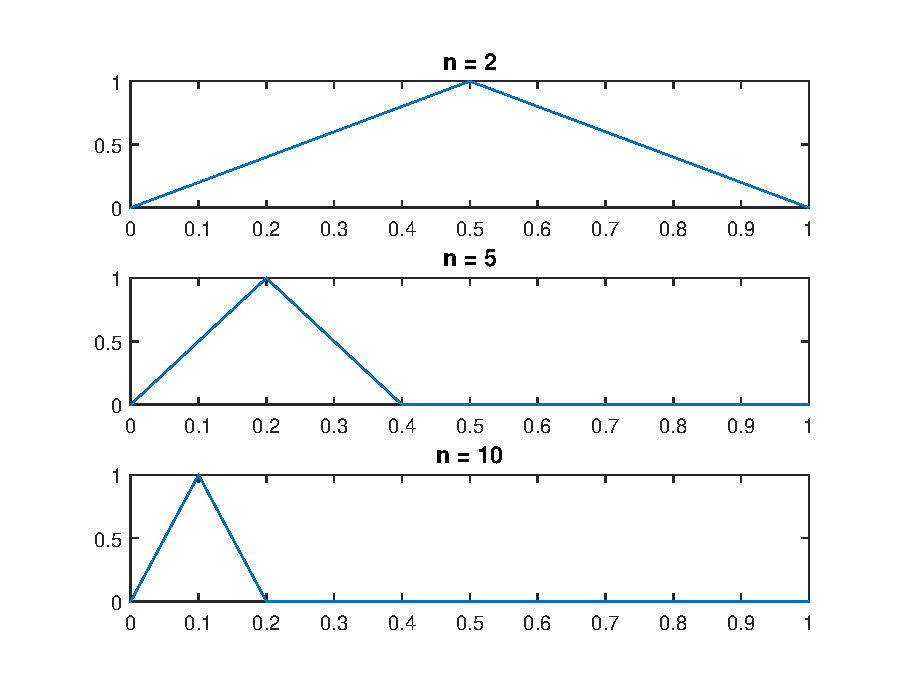
\includegraphics[width=1\textwidth]{../ex1/hatplot}
	\caption{Here we can see how the hat function behave for different values of n.}
	\label{fig:hatplot}
\end{figure}

To continue we have plotted the linear interpolant $\pi  f \in V_h$ of $f(x) = x(1-x)$ as defined by
\begin{equation}
	 \pi f(x) = \Sigma^n_{i=1} f(x_i) \phi_i(x)
	 \label{eq:inter}
\end{equation}
Which basically is just plotting the values of f(x) at certain points and dragging a straight line in between them. We illustrate this is figure \ref{fig:inter} for different amounts of points $n$. 
\begin{figure}[H]
	\centering
	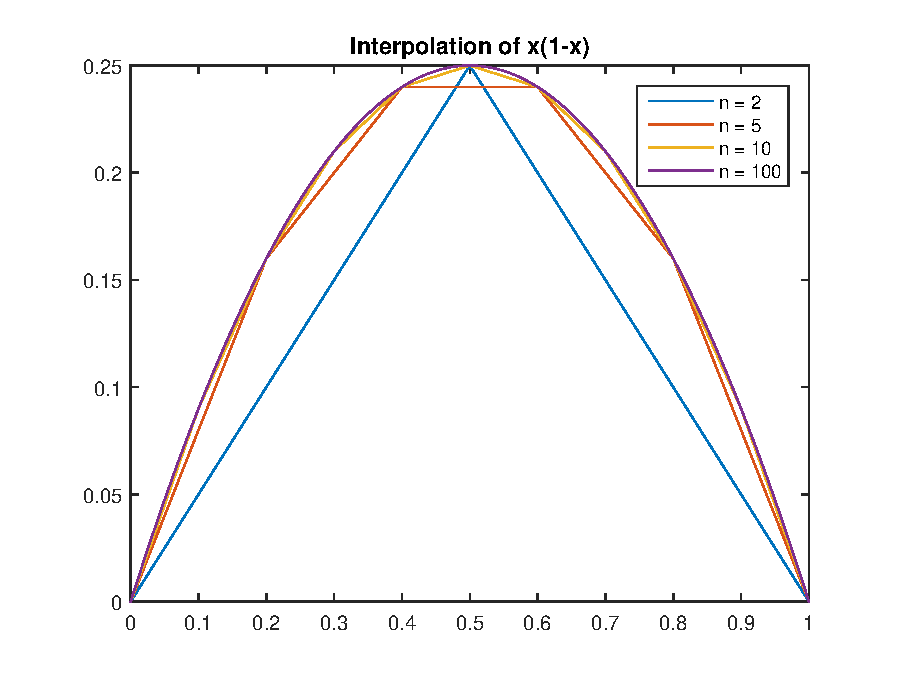
\includegraphics[width=1\textwidth]{../ex1/inter}
	\caption{An interpolation as described in equation \ref{eq:inter} for different values on $n$.}
	\label{fig:inter}
\end{figure}

In appendx \label{code:L2mass1D} we can see how the mass matrix for solving the $L^2$-projection problem was implemented. We use this mass matrix to calculate the $L^2$ projection $P_h f \in V_h$ of $f(x) = x(1-x)$. But to create the load vector for the problem we use two methods. The different values $b_i$ of the load vector $\bar{b}$ are basically 
\begin{equation}
	b_i = \int_{x_i - 1}^{x_i} f(\phi_i) dx + \int_{x_i}^{x_i+1} f(\phi_i) dx.
\end{equation}
In order to estimate these values we use either trapezoidal or simpsons method in this lab. The code for the code creating the load vector using the trapezoidal method is in appendix \ref{code:L2Load1D}, the code for the simpsons is in appendix \ref{code:LoadAssemblerS1D}. Looking at figure \ref{fig:l2proj} we can see how much better the values look like if one use the simpsons method to assemble the load vector compared to the trapezoidal. But one should not stop looking there. If we compare figure \ref{fig:inter} to \ref{fig:l2proj} we can see how the estimation methods differ. It is clear from figure \ref{fig:inter} that the first method we used tend to low ball the function and if you where to integrate the estimation the value would come out consistently low\footnote{This would of course balance itself out if one where to do this estimation on say a sinus function that evenly goes up and down for infinity.}. Looking at figure \ref{fig:l2proj} we can instead see how the values goes over and under the correct values, thus given a more correct value, balanced around the correct one,  if one where to integrate the estimated function. This is natural since how the $L^2$ projection uses integral signs in the estimation. 
\begin{figure}[H]
	\centering
	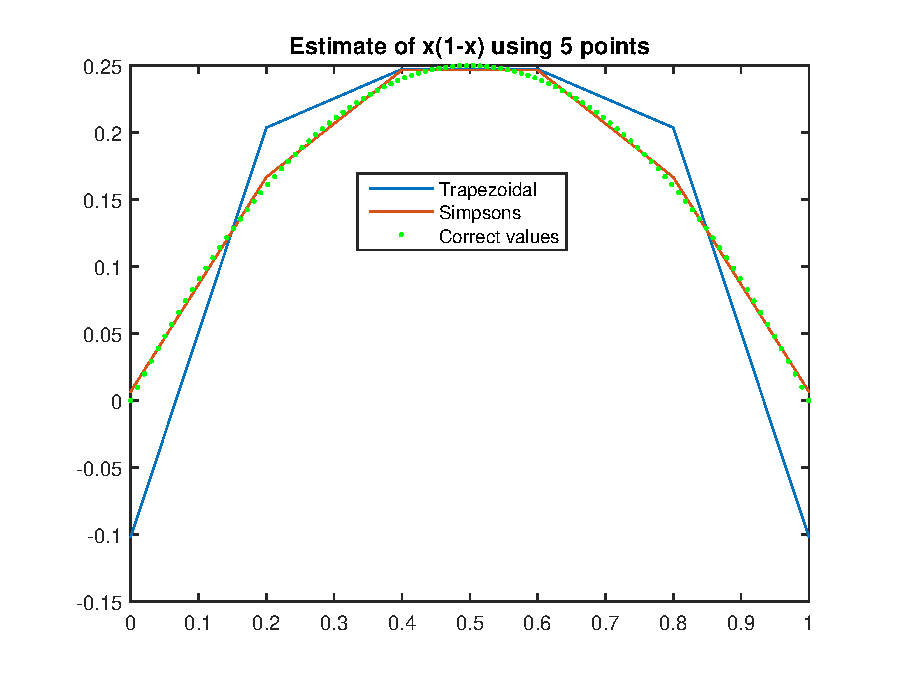
\includegraphics[width=1\textwidth]{../ex1/l2proj}
	\caption{Showing how the different approaches to the load vector assembly yeild different results.}
	\label{fig:l2proj}
\end{figure}

\section{Problem 2}
In this exersice we solve the initial value problem $-u'' = 2,0<x<1,u(0)=u(1)=0$. We us a uniform mesh with the step size $h = 1/2, 1/4, 1/16, 1/256$. 
\begin{figure}[H]
	\centering
	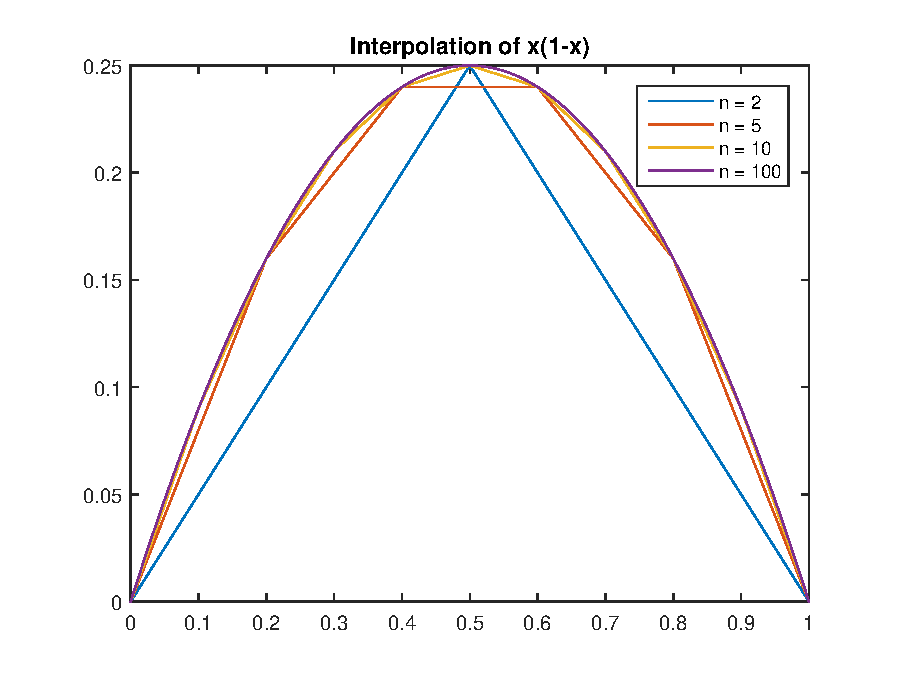
\includegraphics[width=1\textwidth]{../ex1/inter}
	\caption{An interpolation as described in equation \ref{eq:inter} for different values on $n$.}
	\label{fig:inter}
\end{figure}





\appendix
\section{Code for Problem 1}
\subsection{hatfun}\label{code:hatfun}
\verbatimtabinput{../ex1/hatfun.m}

\subsection{L2Mass1D}\label{code:L2Mass1D}
\verbatimtabinput{../ex1/L2Mass1D.m}

\subsection{L2Load1D}\label{code:L2Load1D}
\verbatimtabinput{../ex1/L2Load1D.m}

\subsection{LoadAssemblerS1D}\label{code:LoadAssemblerS1D}
\verbatimtabinput{../ex1/LoadAssemblerS1D.m}
\end{document}
